\documentclass[a4paper,10pt, sans]{article}
\usepackage[utf8x]{inputenc}
\usepackage[spanish]{babel}
\usepackage{hyperref}
\usepackage{verbatim}
\usepackage{graphicx}
\usepackage{float}
\usepackage{wrapfig}
\usepackage{ltxtable}
%\usepackage{amsmath,amssymb,amsfonts,latexsym,cancel}
\usepackage{multicol}      %para usar varias columnas
  %uso:
  %\begin{multicols}{2}
    %texto
  %\end{multicols}
\usepackage{marvosym}

\setlength{\columnsep}{4mm}    %separación de columnas
%\usepackage{pslatex}
%\hoffset -0.75in        %cambio el margen horizontal izquierdo
%\voffset -0.9in          %cambio el margen vertical superior
\textwidth 17cm        %ancho de texto. defaut: 14cm
\textheight 25cm        %alto de texto. default: 19cm
\topmargin -1cm        %agranda el margen superior. default: 3cm
\oddsidemargin -1cm        %agranda el margen izquierdo. default: 2.5cm (4.5 si no aparece esta instrucción)
\pagestyle{empty} %{myheadins}  %numeración de pág: sin / arriba
\parskip 2mm          %X mm entre párrafos
%\parindent 0mm          %elimina sangría

\begin{document}
  

\begin{wrapfigure}{r}{4cm}
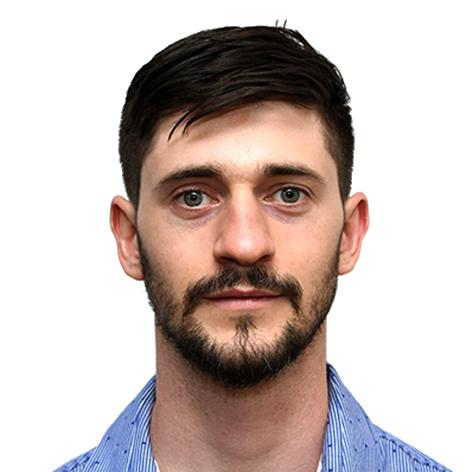
\includegraphics[height=4cm]{seba_4x4.jpg}
\end{wrapfigure}

\sffamily

\begin{Huge}
Sebastián Rossi
\end{Huge}
\\ \\
\hspace*{0.5cm} \textit{CURRICULUM VITAE} \\
\hspace*{0.5cm} \textit{Actualizado: 30/05/2023}

\begin{tabular}{rl}
\vspace{0.5cm} \\
\large\Mobilefone & \textbf{+549 3402 507471} \\
\large\Letter & \textbf{srossi@inti.gob.ar}
\end{tabular}

\vspace{0.5cm}
\large
\begin{table}[H]
  \begin{tabularx}{\textwidth}{r X}
    %%%%%%%%%%%%%%%%%%%%%%%%%%%%%%%%%%%%%%%%%%%%%%%%%%%%%%%%%%%%%%%%%%%%%%%%%%%% \hline \\
    \textbf{Datos Personales} & {} \\
      {} & DNI: 34171919 \\
      {} & Fecha de nacimiento: 15 de Noviembre de 1988 \\
      {} & Lugar de nacimiento: Álvarez, Santa Fe \\
      {} & Nacionalidad: Italiano - Argentino \\
      {} & Estado Civil: Soltero \\
      {} & Domicilio: Maipú 782, Álvarez, Santa Fe \\ \\ \hline \\
    %%%%%%%%%%%%%%%%%%%%%%%%%%%%%%%%%%%%%%%%%%%%%%%%%%%%%%%%%%%%%%%%%%%%%%%%%%%%
\end{tabularx}
\end{table}

\begin{table}[H]
\begin{tabularx}{\textwidth}{r X}         
    \textbf{Educación} & {} \\ [1ex]
       (2020 - ) & \textbf{Doctorado en Ingeniería}, FCEIA, Universidad Nacional de Rosario. Tesis: Sensado y control de sistemas de siembra neumáticos. Directores: Ignacio Rubio Scola, Gastón Bourges.\\ [1ex]
       (2008 - 2014) & \textbf{Ingeniero Electrónico}. FCEIA, Universidad Nacional de Rosario.\\ \\ \hline \\
    %%%%%%%%%%%%%%%%%%%%%%%%%%%%%%%%%%%%%%%%%%%%%%%%%%%%%%%%%%%%%%%%%%%%%%%%%%%%
    \textbf{Experiencias} & {} \\ [1ex]
      {} & (2007) RIAM Ascensores. \\
      {} & Montaje y mantenimiento de ascensores (pasantía de tres meses). \\ \\
      {} & (2013 - Actualidad) INTI (Instituto Nacional de Tecnología Industrial). \\
      {} & Legajo: 28202. \\
      {} & Departamento de Ingeniería de Productos Industriales Región Centro.\\ \\
              
        {} &  \textit{Trabajos realizados para el centro INTI -Rosario.} \\
        {} & (2013) Estudio de distribución de temperaturas y tiempos de establización térmica en laboratorio de calibración de bloques patrones  para determinar su efecto en la incertidumbre informada. \\
        {} & (2013 - 2014) Desarrollo de software para la adquisición de datos por puerto serie de comparadora de bloques patrones según requisitos de laboratoristas. \\
        {} & (2014 - 2015) Desarrollo e implementación de sistema de grabación multicanal comandado por Wi-Fi con placas de desarrollo Raspberry Pi. Aplicaciones: Detección de impacto de semillas. \\
        {} & (2015 - 2016) Desarrollo de scripts en Scilab para procesar grabaciones de impactos de diferentes tipos de semillas para determinación de tiempos de impacto y evaluación de sistemas de siembra según norma ISO 7256 (parte 1 para siembra de precisión y parte 2 para siembra a chorrillo). \\
        {} & (2016) Desarrollo de scrit en Matlab para determinar trayectorias de semillas en filmaciones con cámara de alta velocidad. \\
        {} & (2016) Diseño y construcción de prototipo de soporte para cortar pilas, requerido por laboratorio de alimentos y ambiente. \\
        {} & (2016) Participación en la determinación de las especificaciones de los equipos y transductores requeridos en el área diseño y desarrollo. \\
\end{tabularx}
\end{table}

\begin{table}[H]
\begin{tabularx}{\textwidth}{r X}  
 \textbf{Experiencias} & {} \\ [1ex]
        {} & (2016 - 2017) Redacción de documentación para integrar el servicio de medición con galgas extensiométricas al sistema de gestión de la calidad. \\
        {} & (2016 - 2017) Desarrollo e implementación de caja de resistencias para calibración del equipo adquisidor de datos para medición con galgas extensiométricas. \\
        {} & (2016 - 2017) Desarrollo de sistema de detección de impacto de semillas en plataforma con microcontrolador Cortex M4 para aumentar la cantidad de canales sincronizados de adquisición. \\
        {} & (2017) Evaluación de diferentes sensores alternativos para la detección de semillas. Construcción de un prototipo de arreglo de sensores de fuerza. \\
        {} & (2017) Diseño de placa electrónica para registrador de temperatura, presión y humedad desarrollado en INTI Rosario. \\
        {} & (2017) Ensayos en banco de pruebas de dosificador tipo air-drill para evaluar comportamiento con diferentes configuraciones de torta distribuidora y diferentes caudales de aire. \\
        {} & (2018) Desarrollo de dispositivos electrónicos para adquisición de datos y transmisión de datos inalámbrica para cubrir necesidades de medición a campo de presión e impacto de semillas en múltiples cuerpos de siembra. \\
        {} & (2019) Ensayos en banco de pruebas de dosificador tipo air-drill para evaluar comportamiento con diferentes configuraciones de torta distribuidora, diferentes caudales de aire y diferentes combinaciones de longitudes de mangueras de salida aplicando ``definitive screening design''. \\
        {} & (2019) Mejoras en sustracción de fondo e identificación de trayectorias en software de detección de trayectorias de semillas en videos desarrollado en INTI. \\
        {} & (2020) Redacción de publicación sobre sistema de evaluación de dosificadores de siembra en mesa vibratoria con análisis de imágenes. \\
        {} & (2020) Análisis de datos de ensayos Air-drill 2019 y redacción de publicación. \\
        {} & (2020) Experimento en banco estático para evaluación de incertidumbre de sistemas de detección de semillas y trayectorias con placa de impacto y procesamiento de imágenes.\\
        {} & (2021) Mejoras en software de detección de trayectorias por análisis de imágenes y evaluación de incertidumbre. \\
        {} & (2021) Programación de script para análisis estadístico de datos obtenidos por procesamiento de imágenes en Julia. \\ \\

        {} & ~ \textit{Trabajos realizados para usuarios del INTI.} \\
        {} & (2015 - 2016) Evaluación de sistema de siembra para empresa Indecar. Mediciones de detección de semillas en banco de pruebas y en diferentes puntos de la sembradora trabajando en campo. \\
        {} & (2015 - 2016) Evaluación de sistema de siembra para empresa Siembra Neumática. Mediciones de detección de semillas en banco de pruebas y filmación de caida de semillas en tubo de descarga para evaluar trayectorias. \\
        {} & Pegado de galgas extensiométricas y medición de deformaciones en semirremilque para empresa Sola y Brusa. \\
        {} & (2016) Pegado de galgas extensiométricas y medición de deformaciones en estructura soporte de planta potabilizadora móvil del Ejército Argentino. \\
        {} & (2017) Ensayos en sistema de siembra para la empresa Siembra Neumática. Evaluación de desempeño de diferentes modelos de enrasadores. Evaluación de desempeño de diferentes tapas del dosificador. Evaluación de desempeño de diferentes discos dosificadores. Pruebas realizadas en banco de ensayo con placa de detección de semillas y filmación con cámara de alta velocidad de obturación. \\
        {} & (2017) Pegado de galgas extensiométricas y medición de deformaciones en paragolpes Ombú ensayado en INTI Costrucciones. \\
        {} & (2018) Pegado de galgas extensiométricas y medición de deformaciones en tren trasero de fumigadora Pla. \\
        {} & (2018) Medición de presiones en cabina de fumigadora Pla. \\
        {} & (2018) Ensayos en sistema de siembra para la empresa Siembra Neumática. Evaluación de desempeño de diferentes formas en corte de vacío. Evaluación de dosificador Nova Siembra. Filmación con cámara de alta velocidad y detección de trayectorias para evaluación de diferentes tubos de descarga (experimento screening). \\
\end{tabularx}
\end{table}

\begin{table}[H]
\begin{tabularx}{\textwidth}{r X}  
 \textbf{Experiencias} & {} \\ [1ex]
        {} & (2018) Pegado de galgas extensiométricas y medición de deformaciones en sembradora Superwalter. \\
        {} & (2019) Pegado de galgas extensiométricas y medición de deformaciones en batea volcable Ombu. \\
        {} & (2019) Pegado de galgas extensiométricas y medición de deformaciones en cuerpos de enganche de vagón de Acerías 4C en máquina de tracción. \\
        {} & (2019) Ensayos en sistema de siembra para la empresa Siembra Neumática. Filmación con cámara de alta velocidad y detección de trayectorias para evaluación de diferentes tubos de descarga. Experimento definitivo estático y experimento dinámico en mesa vibratoria.  \\
        {} & (2021) Pegado de galgas extensiométricas y medición de deformaciones en dos modelos de sembradoras Crucianelli. \\
        {} & (2021) Pegado de galgas extensiométricas y medición de deformaciones en sembradora Agrometal. \\
        {} & (2021) Ensayos en sistema de siembra para la empresa Agrometal. Filmación con cámara de alta velocidad y detección de trayectorias para evaluación de diferentes variedades de maíz, inclinaciones y velocidad de avance. Experimento estático y dinámico en mesa vibratoria. \\
\end{tabularx}
\end{table}

\begin{table}[H]
\begin{tabularx}{\textwidth}{r X}  
 \hline \\
    %%%%%%%%%%%%%%%%%%%%%%%%%%%%%%%%%%%%%%%%%%%%%%%%%%%%%%%%%%%%%%%%%%%%%%%%%%%%
    \textbf{Cursos} & {} \\ [1ex]
      {} & CCNA Exploration 1 y 2 (Cisco). \\ 
      {} & Evaluación de incertidumbre de medición. \\
      {} & ~ Duración: 16 hs. INTI-Rosario. \\ 
      {} & Automatización de pruebas unitarias y de integración en el desarrollo del software. \\
      {} &   ~ Duración: 21 hs. INTI-Córdoba. \\ 
      {} & Testing embebido con metodologías ágiles. \\
      {} &   ~ Duración: 21 hs. INTI-Córdoba. \\ 
      {} & Solidworks. \\
      {} &  ~ Duración: 24 hs. Disegno Soft SRL. \\ 
      {} & Análisis de vibraciones, categoría II, ISO 18436-2. \\
      {} & ~ Duración: 38 hs. Semapi Argentina S.A. \\ 
      {} & Programación de microcontroladores PIC en lenguaje C. \\
      {} & ~ Duración: 30 hs. Escuela de posgrado de la FCEIA - UNR. \\
      {} & Síntesis de sistemas digitales en FPGA. \\
      {} & ~ Duración: 30 hs. Escuela de posgrado de la FCEIA - UNR. \\
      {} & RTOS sobre microcontroladores de 32 bits. \\
      {} & ~ Duración: 30 hs. Escuela de posgrado de la FCEIA - UNR. \\
      {} & Diseño​ ​de​ ​circuitos​ ​impresos​ ​con​ ​el​ ​software​ ​libre​ ​KiCAD. \\
      {} & ~ Duración: 6 hs. Workshop en SASE 2017. \\
      {} & Diseño de experimentos. \\
      {} & ~ Duración 30 hs. Escuela de posgrado de la FCAGR - UNR. \\
      {} & Análisis multivariado. \\
      {} & ~ Duración: 50 hs. Escuela de posgrado de la FCAGR - UNR. \\
      {} & Introducción al diseño y análisis de experimentos. \\
      {} & ~ Duración: 38 hs. Escuela de graduados y extensión universitaria de la FCECON - UNR. \\
      {} & Procesamiento digital de imágenes. \\
      {} & ~ Duración: 70 hs. Escuela de posgrado de la FCEIA - UNR. \\
      {} & Modelado y simulación de sistemas dinámicos. \\
      {} & ~ Duración: 70 hs. Escuela de posgrado de la FCEIA - UNR. \\ \\ \hline \\
\end{tabularx}
\end{table}

\begin{table}[H]
\begin{tabularx}{\textwidth}{r X}  
    \textbf{Publicaciones} & {} \\ [1ex]
      {} & Gastón Bourges, Sebastian Rossi, Jorge Eliach, Mabel Azucena Medina. \textit{Evaluación experimental de un dosificador de semillas de precisión.} V CAIM 2016. Santiago del Estero, Argentina. UNSE- FCEyT- ISBN: 978-987-1676-63-7. pp: 881-891. \\  [1ex]
      {} & \textit{Ensayos en un dosificador de sembradoras de precisión.} X Jornadas de Ciencia y Tecnología, 2016. Sede de Gobierno. UNR. Rosario, Santa Fe. \\  [1ex] 
\end{tabularx}
\end{table}

\begin{table}[H]
\begin{tabularx}{\textwidth}{r X}  
    \textbf{Publicaciones} & {} \\ [1ex]
      {} & Sebastián Rossi, Ignacio Rubio Scola,Jorge J. Eliach, Gastón Bourges. \textit{Evaluación de desempeño de dosificador monograno mediante filmación y procesamiento de imágenes.} VII CAIM 2020. San Nicolás, Argentina. ISBN 978-950-42-0210-3. \\  [1ex]
      {} & Gastón Bourges, Sebastián Rossi, Ignacio Rubio, Davut Karayel. \textit{Evaluación de la incidencia de diferentes factores en la distribución de semillas de soja en sistema de transporte por aire.} VII CAIM 2020. San Nicolás, Argentina. ISBN 978-950-42-0210-3. \\ [1ex]
      {} & Ignacio Rubio Scola, Sebastián Rossi, Gastón Bourges. \textit{Air drill Seeder Distributor Head Evaluation: A Comparison between Laboratory Tests and Computational Fluid Dynamics Simulations.} Capítulo de libro: Information and Communication Technologies for Agriculture—Theme II: Data. https://doi.org/10.1007/978-3-030-84148-5\_8. \\ \\ \hline \\
\end{tabularx}
\end{table}

\begin{table}[ht!]
\begin{tabularx}{\textwidth}{r X}  
 \hline \\
    %%%%%%%%%%%%%%%%%%%%%%%%%%%%%%%%%%%%%%%%%%%%%%%%%%%%%%%%%%%%%%%%%%%%%%%%%%%%
    \textbf{Lengua extranjera} & {} \\ [1ex]
      {} & Inglés: ~ Nivel B2. \\ \\
 \hline \\
    %%%%%%%%%%%%%%%%%%%%%%%%%%%%%%%%%%%%%%%%%%%%%%%%%%%%%%%%%%%%%%%%%%%%%%%%%%%%
    \textbf{Conocimientos Informáticos} & {} \\ [1ex]
      {} & Office. \\
      {} & Conocimiento básico de linux. \\
      {} & Lenguajes de programación: C, matlab, python, R, scilab, Modelica, Julia. \\ 
      {} & Autocad. \\
      {} & Solid Works. \\ \\
 \hline \\
    %%%%%%%%%%%%%%%%%%%%%%%%%%%%%%%%%%%%%%%%%%%%%%%%%%%%%%%%%%%%%%%%%%%%%%%%%%%%
    \textbf{Documentación Adicional} & {} \\ [1ex]
      {} & Carné de conducir, clase A3, B2.
  \end{tabularx}
\end{table}

\end{document}
